\textbf{Cas d'utilisation:} Paie le passage

\textbf{Acteur primaire:} Conducteur

\textbf{Acteur support:} Le poste de surveillance et opérateur humain(si le borne est manuelle)

\textbf{Pré-condition: }  la borne est opérationnelle
%La borne affiche le montant 
%La boucle au sol détermine la présence du véhicule
 
%\textbf{Post-condition: } 

\textbf{Scenario primaire: } \\
    \textbf{1.} La borne attende le conducteur choisir un moyen de payment accepté pour le borne\\
    %La borne affiche le montant \\ %Le conducteur insère le moyen de paiement. cesaaaar
    \textbf{2.} Le conduteur paier avec carte bleu (\ref{subsec:paierBleu})\\
    \textbf{3.} Paiement etait accepté. Le feu change de couleur\\

\textbf{Variantes:}\\
    \textbf{2a.} Le conduteur paier par liquide (\ref{subsec:paieLiquide})\\
    \textbf{2b.} Le conduteur paier avec cart abonnement (\ref{subsec:paierAbonement})\\
    \textbf{2c.} Le conduteur ne peut pas payer \\ %he clicks in the botton who calls the technicien 

%IMAGES
\textbf{Décomposition des cas d'utilisation:} 
\begin{figure}[h]
    \centering
    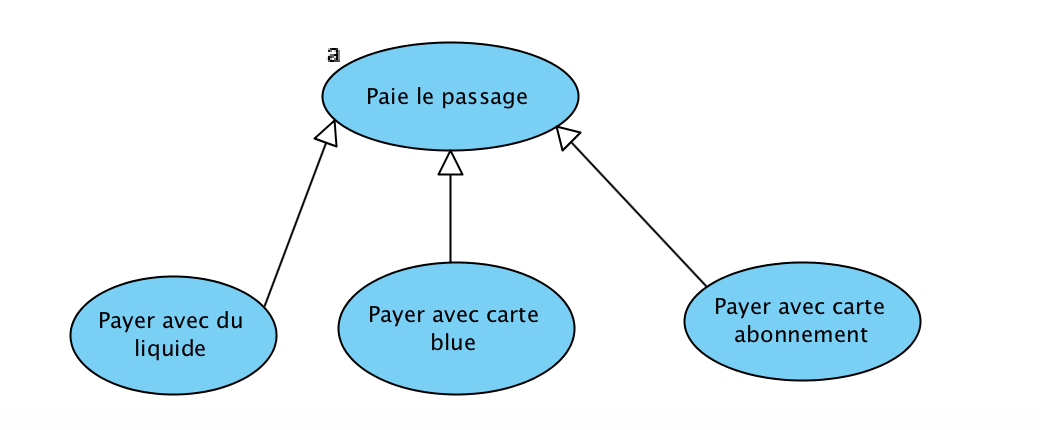
\includegraphics[scale=0.7]{02_Desenvolvimento/TD2/images/paierInclusion.png}
    \caption{Décomposition des cas d'utilisation: Paie le passage}
\end{figure}